\section{Examples}
In this section we present a set of minimal examples 
that demonstrate how to use Pigeons.jl for sampling. 
We also direct readers to our growing list of examples at InferHub 
(\url{https://julia-tempering.github.io/InferHub/}), which hosts a  collection of posterior 
distributions with an emphasis on difficult (non-log-concave) problems.


We begin by installing the latest official release of Pigeons.jl: 
\begin{lstlisting}[language = Julia]
using Pkg; Pkg.add("Pigeons")
\end{lstlisting}


\subsection{Targets}
To use Pigeons.jl, we must specify a target distribution, given by $\gamma$ 
in \cref{eq:normalizing_constant}.
Numerous possible types of target distributions are supported, including 
custom probability densities (specified up to a normalizing constant) written in Julia.
We also allow to interface with models written in common probabilistic programming 
languages, including:
\begin{itemize}
    \item Turing.jl \cite{ge2018turing} models (\texttt{TuringLogPotential})
    \item Stan \cite{carpenter2017stan} models (\texttt{StanLogPotential})
    \item Comrade.jl\footnote{\url{https://github.com/ptiede/Comrade.jl}} 
      models for black hole imaging (\texttt{ComradeLogPotential})
    \item Non-Julian models with foreign-language Markov chain Monte Carlo (MCMC) code 
    (e.g. Blang \cite{bouchard2022blang} code for phylogenetic inference over combinatorial spaces) 
\end{itemize}
Additional targets are currently being accommodated and will be 
introduced to Pigeons.jl in the near future.

 
In what follows, we demonstrate how to use Pigeons with a Julia Turing model 
applied to a non-identifiable ``coinflip'' data set.
The Bayesian model can be formulated as 
\[
  \label{eq:coinflip}
  p_1, p_2 &\stackrel{\text{i.i.d.}}{\sim} U(0, 1), \\    
  y \mid p_1, p_2 &\sim \text{Binomial}(n, p_1 p_2).
\]
The random variable $y$ is the number of heads observed on $n$ coin flips
where the probability of heads is $p_1 p_2$.  
This model is non-identifiable, meaning that it is not possible to distinguish 
the effects of the two different parameters $p_1$ and $p_2$. As a consequence, 
the target distribution exhibits a complicated structure, as displayed in 
\cref{fig:coinflip_posterior}.
The density of interest corresponding to this model is 
\[
  \pi(p_1, p_2) &= \gamma(p_1, p_2)/Z,
\] 
where 
\[ 
  \gamma(p_1, p_2) &= 
    \binom{n}{y} (p_1 p_2)^y (1-p_1 p_2)^{n-y} I[p_1, p_2 \in [0,1]] 
    \label{eq:coinflip_density} \\
  Z &= \int_0^1 \int_0^1 \gamma(p_1, p_2) \, \dee p_1 \, \dee p_2. \label{eq:coinflip_normalization}
\]
The distribution $\pi$ is also known as the \emph{posterior distribution} in 
Bayesian statistics.

\begin{figure}[t]
    \centering 
    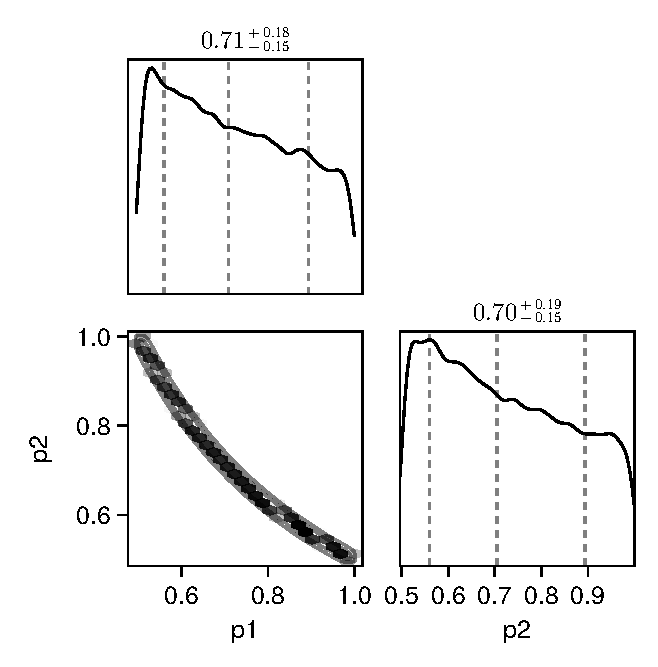
\includegraphics[width=0.8\linewidth]{../img/coinflip_posterior.pdf}
    \caption{Posterior distribution for the model given by \cref{eq:coinflip} 
    with $n=100,000$ coin flips and $y=50,000$ observed heads, 
    estimated using $2^{17}$ samples from Pigeons.jl. 
    We present the pairwise plot for $p_1$ and $p_2$, as well as the estimated 
    densities of the marginal of the posterior for each of the two parameters.
    Note that because the model is non-identifiable, as we collect more data the 
    posterior distribution concentrates around the curve $p_1 p_2 = 0.5$, instead 
    of a single point, assuming that the true probability of observing heads 
    is 0.5.}
    \label{fig:coinflip_posterior}
\end{figure}

 
Suppose that we perform $n=100,000$ coin tosses and observe 
$y=50,000$ heads.
We would like to obtain samples from our posterior, $\pi$, having collected this data.
We begin by installing Turing
\begin{lstlisting}[language = Julia]
Pkg.add("Turing")
\end{lstlisting}
and then defining our Turing model and storing it in the variable \texttt{model}:
\begin{lstlisting}[language = Julia]
using Turing
@model function coinflip(n, y)
    p1 ~ Uniform(0.0, 1.0)
    p2 ~ Uniform(0.0, 1.0)
    y ~ Binomial(n, p1 * p2)
    return y
end
model = coinflip(100000, 50000)
\end{lstlisting}

From here, it is straightforward to sample from the density given by 
\cref{eq:coinflip_density} up to a normalizing constant.
We use non-reversible parallel tempering 
\cite{syed2021nrpt,syed2021paths,surjanovic2022vpt,surjanovic2024ergodicity} (PT), Pigeons.jl's 
state-of-the-art sampling algorithm, to sample from the target distribution.
PT comes with several tuning parameters and \cite{syed2021nrpt} describe how 
to select these parameters effectively, which Pigeons.jl implements under the hood.
We also specify that we would like to store 
the obtained samples in memory to be able to produce trace-plots, as well 
as some basic online summary statistics of the target distribution and useful 
diagnostic output by specifying 
\texttt{record = [traces, online, round\_trip, Pigeons.timing\_extrema, Pigeons.allocation\_extrema]}.
It is also possible to leave the \texttt{record} argument empty and reasonable defaults 
will be selected for the user.
The code below runs Pigeons.jl on one machine with one thread.
We use the default values for most settings, however 
we explain later how one can obtain improved performance by setting 
arguments more carefully (see \cref{sec:additional_options}).
\begin{lstlisting}[language = Julia]
using Pigeons
pt = pigeons(
    target = TuringLogPotential(model), 
    record = [
        traces, online, round_trip, 
        Pigeons.timing_extrema, 
        Pigeons.allocation_extrema])
\end{lstlisting}
Note that to convert the Turing model into an appropriate Pigeons.jl target for sampling, 
we pass the model as an argument to \texttt{TuringLogPotential()}.
Once we have stored the PT output in the variable \texttt{pt} we can 
access the results, as described in the following section. 
For purposes of comparison, we also run a traditional 
(single-chain Markov chain Monte Carlo) method. 


\subsubsection{Other targets}
As mentioned previously, it is also possible to specify targets with custom 
probability densities, as well as Stan and Turing models. 
Additionally, suppose we have some code implementing vanilla MCMC, written 
in an arbitrary ``foreign'' language such as C++, Python, R, Java, etc. 
Surprisingly, it is very simple to bridge such code with Pigeons.jl. 
See \url{https://pigeons.run/stable/input-overview/}.


\subsubsection{Off-memory processing}
When either the dimensionality of the model or the number of samples is large,
the obtained samples may not fit in memory. 
In some cases it may be necessary to store samples to disk if our statistics of 
interest cannot be calculated online and with constant-memory
(see \cref{sec:online_stats}).
We show here how to save samples to disk when Pigeons.jl is run on a single 
machine. A similar interface can be used over MPI. 

 
First, we make sure that we set \texttt{checkpoint = true}, which saves a 
snapshot at the end of each round in the directory \texttt{results/all/<unique directory>}
and is symlinked to \texttt{results/latest}.
Second, we make sure that we use the \texttt{disk} recorder 
by setting \texttt{record = [disk]}, along with possibly any other desired recorders.
Accessing the samples from disk can then be achieved in a simple way using the Pigeons.jl 
function \texttt{process\_sample()}.


\subsubsection{PT diagnostics}
\label{sec:PT_diagnostics}
We describe how to produce some key parallel tempering diagnostics from 
\cite{syed2021nrpt}.

 
The global communication barrier, denoted $\Lambda$ in Pigeons.jl output, can be 
used to approximately inform the appropriate number of chains. 
Based on \cite{syed2021nrpt}, stable PT performance should be achieved when  
the number of chains is set to roughly $2\Lambda$. This can be achieved by 
modifying the \texttt{n\_chains} argument in the call to \texttt{pigeons()}. 
The global communication barrier is shown at each round and can also be accessed 
with 
\begin{lstlisting}[language=Julia]
Pigeons.global_barrier(pt)
\end{lstlisting}

The number of restarts per round can be accessed with 
\begin{lstlisting}[language=Julia]
n_tempered_restarts(pt)
\end{lstlisting}
These quantities are also displayed in \cref{fig:standard_out}. 
Many other useful PT diagnostic statistics and plots can be obtained, as described 
in our full documentation. 


\subsection{Parallel and distributed PT}
One of the main benefits of Pigeons.jl is that it allows users to easily parallelize 
and/or distribute their PT sampling efforts. We explain how to run MPI locally on 
one machine and also how to use MPI when a cluster is available.

\subsubsection{Running MPI locally}
To run MPI locally on one machine using four MPI processes and one thread per process,
use
\begin{lstlisting}[language = Julia]
pigeons(
    target = TuringLogPotential(model), 
    on = ChildProcess(
            n_local_mpi_processes = 4,
            n_threads = 1))
\end{lstlisting}

\subsubsection{Running MPI on a cluster}
Often, MPI is available via a cluster scheduling system. To run MPI over 
several machines:
\begin{enumerate}
    \item In the cluster login node, follow the Pigeons.jl installation instructions
    in our online documentation. 
    \item Start Julia in the login node, and perform a one-time setup by 
    calling \texttt{Pigeons.setup\_mpi()}.
    \item In the Julia REPL running in the login node, run:\footnote{In 
    version 0.4.0 of Pigeons, the function \text{MPI} has been renamed \text{MPIProcesses} 
    to avoid a clash with the library \text{MPI.jl}.}
\end{enumerate}
\begin{lstlisting}[language = Julia]
pigeons(
    target = TuringLogPotential(model), 
    n_chains = 1_000,
    on = MPI(n_mpi_processes = 1_000, 
             n_threads = 1))
\end{lstlisting}
The code above will start a distributed PT algorithm with 1,000 chains on 1,000 
MPI processes each using one thread.
Note that for the above code chunks involving \texttt{ChildProcess()} and 
\texttt{MPI()} to work, it may be necessary to specify dependencies in their 
function calls. See \url{https://pigeons.run/stable/mpi/} for details. 


\subsection{Additional options}
\label{sec:additional_options}
In the preceding example we only specified the target distribution and let 
Pigeons.jl decide on default values for most other settings of the inference engine. 
There are various settings we can change, including: 
the random seed (\texttt{seed}), the number of PT chains (\texttt{n\_chains}), 
the number of PT tuning rounds/samples (\texttt{n\_rounds}), 
and a variational reference distribution family (\texttt{variational}), among other settings.
For instance, we can run 
\begin{lstlisting}[language = Julia]
pigeons(
    target = TuringLogPotential(model),
    n_rounds = 10, 
    n_chains = 10,
    variational = GaussianReference(),
    seed = 2
)
\end{lstlisting}
which runs PT with the same Turing model target as before and explicitly states 
that we should use 10 PT tuning rounds with 10 chains (described below). 
In the above code chunk we also specify that we would like to use a 
Gaussian variational reference distribution.
That is, the reference distribution is chosen from a multivariate Gaussian family 
that lies as close as possible to the target distribution in order to improve 
the efficiency of PT. We refer readers to \cite{surjanovic2022vpt} for more details.
When only continuous parameters are of interest, we encourage users to consider 
using \texttt{variational = GaussianReference()} and setting \texttt{n\_chains\_variational = 10}, 
for example, as the number of restarts may substantially increase with these settings.

